\documentclass{standalone}
\usepackage{tikz}
\usepackage{xcolor}
\definecolor{greeen}{RGB}{34,139,34}
\definecolor{orange}{RGB}{255,165,0}
\usetikzlibrary{arrows,automata}

\begin{document}
    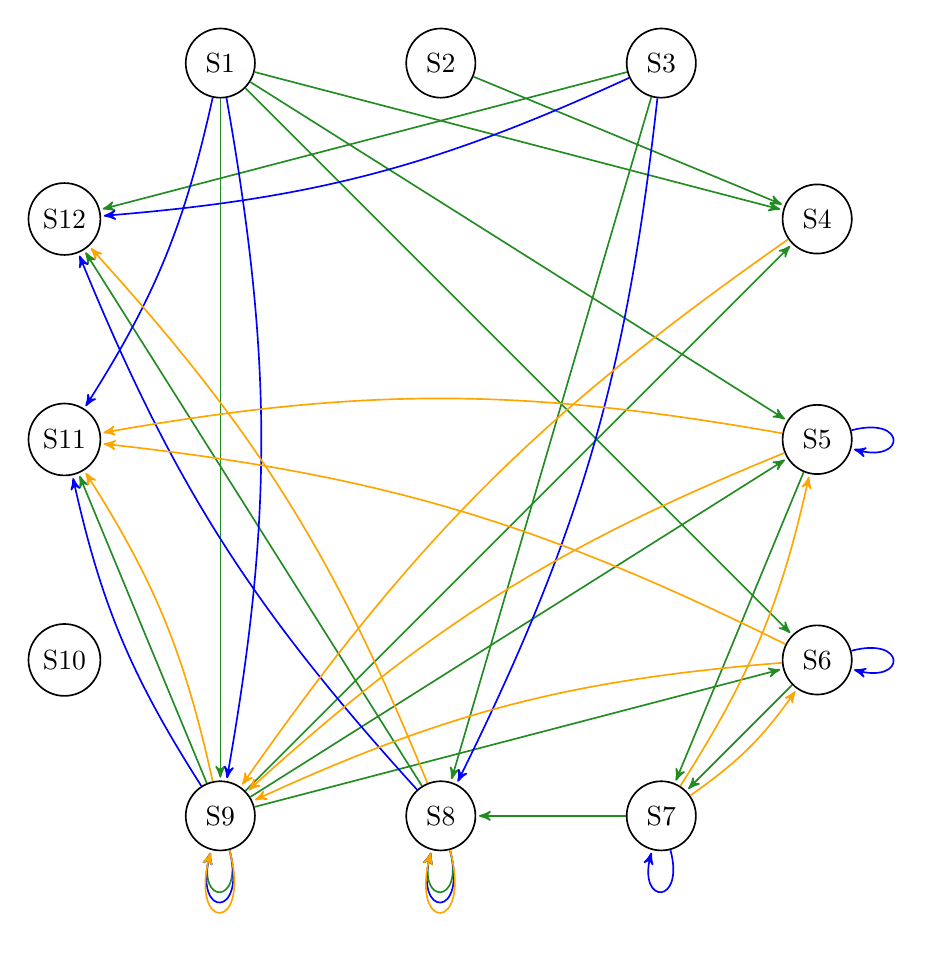
\begin{tikzpicture}[->,>=stealth',shorten >=1pt,auto,node distance=2.8cm,semithick]
        \tikzstyle{every state}=[fill=none,draw=black,text=black]
        \tikzstyle{raw}=[draw=greeen,fill=greeen]
        \tikzstyle{war}=[draw=orange,fill=orange]
        \tikzstyle{waw}=[draw=blue,fill=blue]

        \node[state] (S1)                      {S1};
        \node[state] (S2) [right of=S1]        {S2};
        \node[state] (S3) [right of=S2]        {S3};
        \node[state] (S4) [below right of=S3]  {S4};
        \node[state] (S5) [below of=S4]        {S5};
        \node[state] (S6) [below of=S5]        {S6};
        \node[state] (S12) [below left of=S1]  {S12};
        \node[state] (S11) [below of=S12]      {S11};
        \node[state] (S10) [below of=S11]      {S10};
        \node[state] (S9)  [below right of=S10] {S9};
        \node[state] (S8) [right of=S9]        {S8};
        \node[state] (S7) [right of=S8]        {S7};

        \path[raw]  (S1) edge (S4)
                         edge (S5)
                         edge (S6)
                         edge (S9)
                    (S2) edge (S4)
                    (S3) edge (S8)
                         edge (S12)
                    (S5) edge (S7)
                    (S6) edge (S7)
                    (S7) edge (S8)
                    (S8) edge [loop below] (S8)
                         edge (S12)
                    (S9) edge (S4)
                         edge (S5)
                         edge (S6)
                         edge [loop below] (S9)
                         edge (S11)
        ;
        
        \path[waw]  (S1) edge [bend left=10] (S9)
                         edge [bend left=10] (S11)
                    (S3) edge [bend left=10] (S8)
                         edge [bend left=10] (S12)
                    (S5) edge [loop right] (S5)
                    (S6) edge [loop right] (S6)
                    (S7) edge [loop below] (S7)
                    (S8) edge [loop below, looseness=10] (S8)
                         edge [bend left=10] (S12)
                    (S9) edge [loop below, looseness=10] (S9)
                         edge [bend left=10] (S11)
        ;
        
        \path[war]  (S4) edge [bend right=10] (S9)
                    (S5) edge [bend right=10] (S9)
                         edge [bend right=10] (S11)
                    (S6) edge [bend right=10] (S9)
                         edge [bend right=10] (S11)
                    (S7) edge [bend right=10] (S5)
                         edge [bend right=10] (S6)
                    (S8) edge [loop below, looseness=12] (S8)
                         edge [bend right=10] (S12)
                    (S9) edge [loop below, looseness=12] (S9)
                         edge [bend right=10] (S11)
        ;
    \end{tikzpicture}
\end{document}